% Figure 8: Offline Fallback Chain
% TODO: Replace with actual TikZ diagram showing 4-level fallback strategy

\begin{figure}[htbp]
\centering
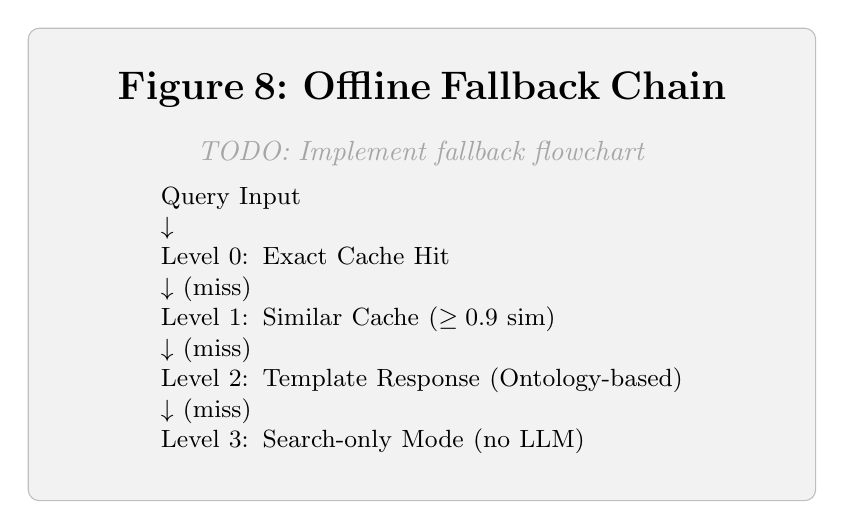
\begin{tikzpicture}
  \node[rectangle, draw=gray!50, fill=gray!10, minimum width=10cm, minimum height=6cm, rounded corners] (placeholder) {};
  \node[text width=9cm, align=center] at (placeholder.center) {
    \textbf{\Large Figure 8: Offline Fallback Chain}\\[1em]
    \textcolor{gray!70}{\textit{TODO: Implement fallback flowchart}}\\[0.5em]
    \small
    \begin{tabular}{l}
    Query Input \\
    $\downarrow$ \\
    Level 0: Exact Cache Hit \\
    $\downarrow$ (miss) \\
    Level 1: Similar Cache ($\geq 0.9$ sim) \\
    $\downarrow$ (miss) \\
    Level 2: Template Response (Ontology-based) \\
    $\downarrow$ (miss) \\
    Level 3: Search-only Mode (no LLM) \\
    \end{tabular}
  };
\end{tikzpicture}
\caption{Four-level fallback strategy enabling offline operation without LLM: exact cache lookup, similar query matching, ontology-based template responses, and search-only mode.}
\label{fig:fallback}
\end{figure}
